\chapter{Anisotropic Image Driven Regularization}
The homogeneous regularizer of Horn and Schunck smoothes the flow field in all directions. Since we are looking for a flow field describing relative movement of objects, the boundary between objects will not have a smooth flow field unless they are moving at the same relative velocity. Methods that reduce the smoothing across image edges are called image-driven regularization methods. The anisotropic reguralizer of Nagel and Enkelmann (1986) performs smoothing along the image gradients and prevents smoothing across image edges. This is done by introducing a regularised projection matrix $P$, defined as
\begin{align*}
P(\nabla f) = \frac{1}{|\nabla f|^2 + 2 \kappa^2} (\nabla^{\bot} f (\nabla^{\bot})^T + \kappa^2 I),
\end{align*}
where $\nabla^{\bot} f= \left[-\frac{\partial f}{\partial y}, \frac{\partial f}{\partial x}\right]^T$, and $\kappa > 0$ is a regularization parameter. The smoothness term of Nagel and Enkelmann can now be written as the following
\begin{align*}
V_{AI}(\nabla u, \nabla v) = \nabla ^T u P(\nabla f) \nabla u + \nabla ^T v P(\nabla f) \nabla v,
\end{align*}
or written out 
\begin{align*}
V_{AI}(\nabla u, \nabla v) = \frac{\kappa^2}{|\nabla f|^2 + 2 \kappa^2} \left( u_{\textbf{s}_1}^2 + v_{\textbf{s}_1}^2 \right) + \frac{|\nabla f|^2 + \kappa^2}{|\nabla f|^2 + 2 \kappa^2} \left(u_{\textbf{s}_2}^2 + v_{\textbf{s}_2}^2 \right),
\end{align*}
where $\textbf{s}_1 = \frac{\nabla f}{|\nabla f|}$, $\textbf{s}_2 = \frac{\nabla^{\bot} f}{|\nabla f|}$ and $q_{\textbf{s}_i} = \textbf{s}_i^T \nabla u$ for $q = u, v$. That is, $q_{\textbf{s}_i}$ is the directional derivative of $q$ in the direction of the image gradient ($i=1$) or the orthogonal direction ($i=2$). This means that setting $D=P$ in (\ref{EL_regu}) steers the diffusion so that flow vectors are smoothed in the direction of the image gradients.

\subsection{Discretizing the Nagel and Enkelmann smoothness term}
Setting $\Theta=P$ in (\ref{EL_regu}) leads to the following Euler-Lagrange system:
\begin{align*}
\frac{\partial M}{\partial u} - \frac{1}{\sigma^2} \text{div}(P \nabla u) = 0 \\
\frac{\partial M}{\partial v} - \frac{1}{\sigma^2} \text{div}(P \nabla v)= 0.
\end{align*}
Using the same discretizations for the derivatives as in \ref{sec: disc} we get the following system:
\begin{align*}
(D^T D + \frac{1}{\sigma^2} L^TPL) \textbf{w} = - D^T \textbf{c}.
\end{align*}

\subsection{Results for the anisotropic image-driven regularization}
Experiments were run to find the best regularization parameter in the Nagel and Enkelmann smoothness term. The regularization parameter $\sigma$ found for the Horn and Schunck method is used to regularize the whole smoothness term. The resulting flow field for different choices of the regularization parameter $\kappa$, while keeping $\sigma$ constant, is shown in Figure (\ref{reguNE}). It is seen that choosing $\kappa = 0.8$ gives a fairly good segmentation of the object. Since the values for the gradient from the sobel derivative are relatively high, it is expected to also having to choose a relatively large value for $\kappa$ for sufficient regularization. Figure (\ref{reguNEHS}) compares the anisotropic smoothness term of Nagel and Enkelmann with $\kappa = 0.8$ with the homogeneous smoothness term of Horn and Schunck, both with using regularization parameter $\sigma = 0.003$. 

%\begin{figure}
%    \centering
%    \includegraphics[scale=0.8]{regularizationNE.eps}
%    \caption{Different choices for $\kappa$ using the Nagel and Enkelmann smoothness term}
%    \label{reguNE}
%\end{figure}
%
%\begin{figure}
%    \centering
%    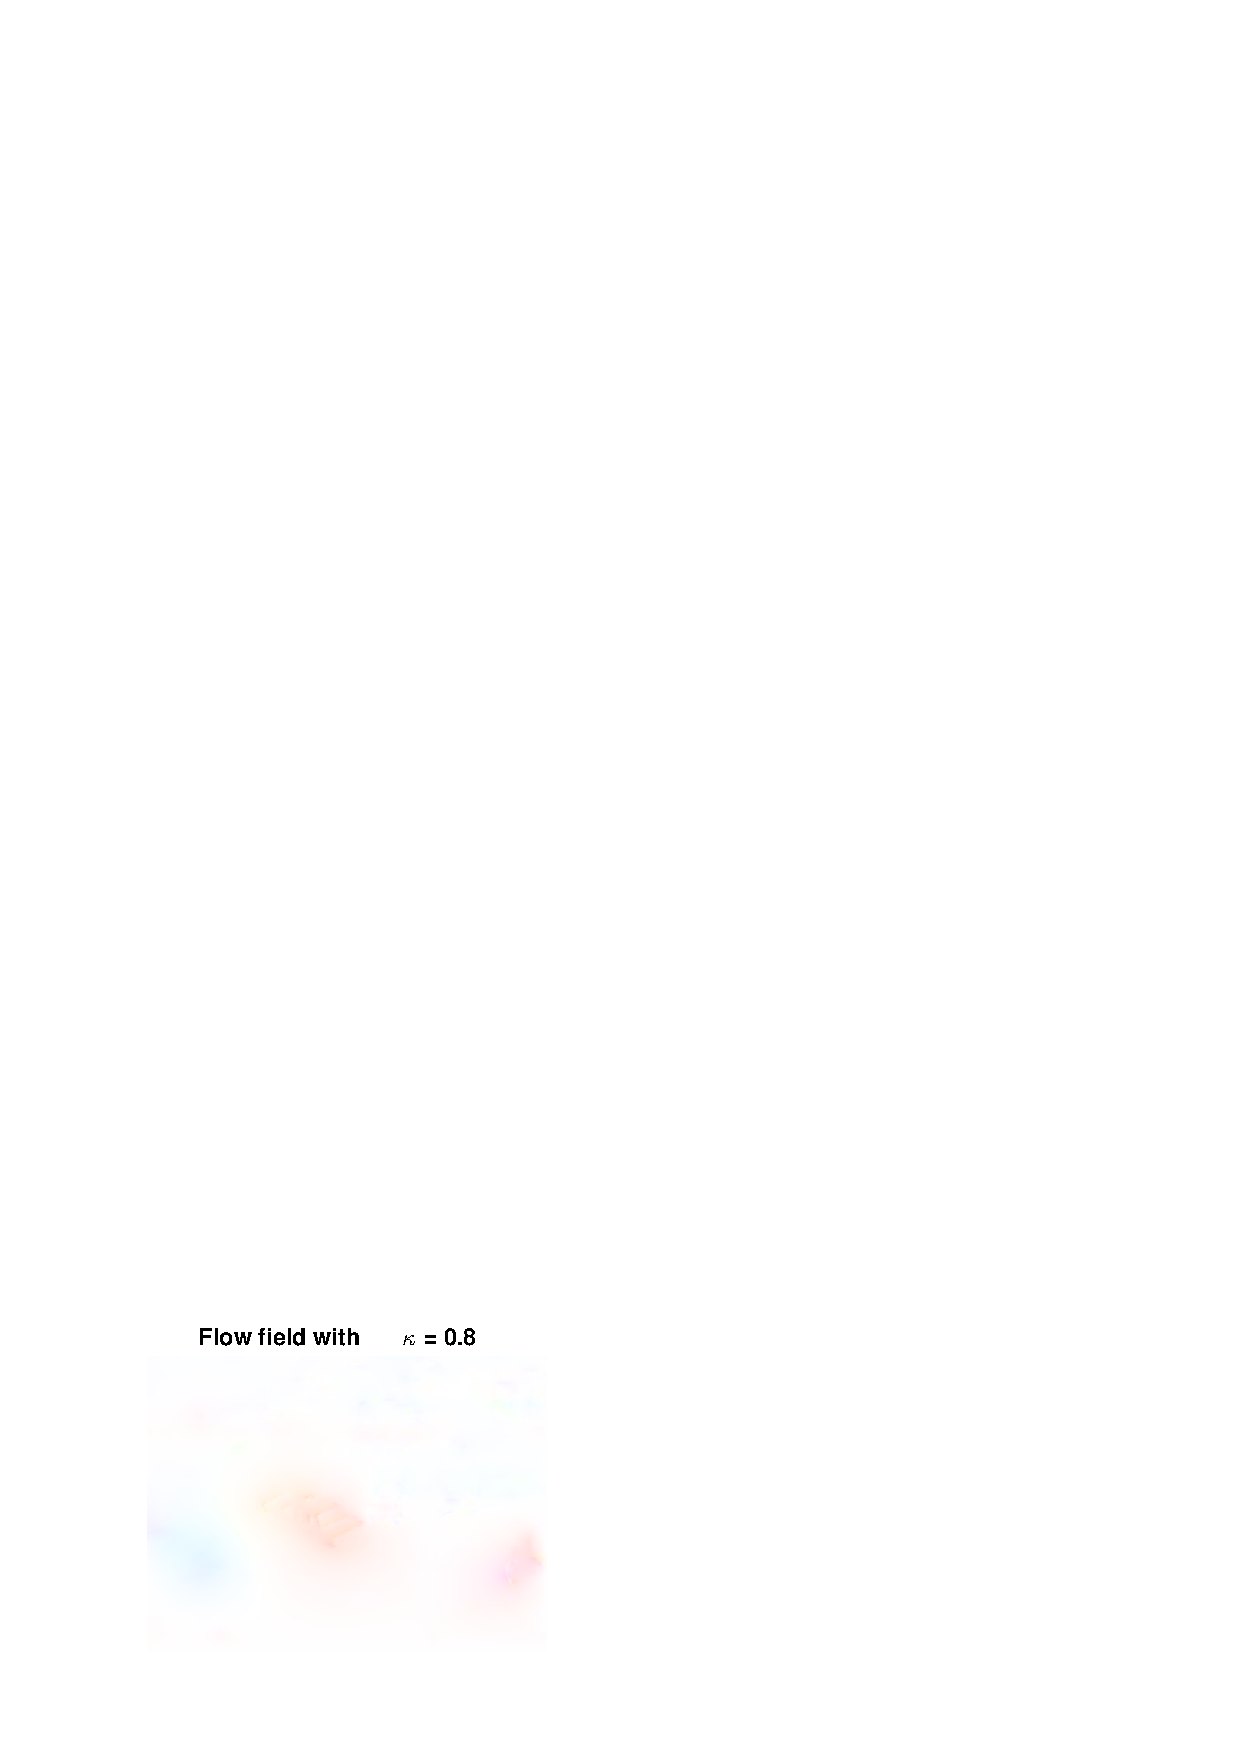
\includegraphics[scale=0.8]{NEregu}
%    \caption{Flow field with $\kappa= 0.8$ and $\sigma = 0.003$ using the Nagel and Enkelmann smoothness term.}
%    \label{reguNE_best}
%\end{figure}
%
%\begin{figure}
%    \centering
%    \includegraphics[scale=0.8]{reguNEHS.eps}
%    \subfloat[\label{NE_best} Anisotropic smoothness term.]{\hspace{.5\linewidth}}
%	\subfloat[\label{HS_best} Homogeneous smoothness term.]{\hspace{.5\linewidth}}
%	\caption{Comparison of the anisotropic and homogeneous smoothness term for given parameter choices.\label{humans}}
%    \label{reguNEHS}
%\end{figure}